\begin{figure}
    \centering
    \resizebox{0.55\textwidth}{!}{%
        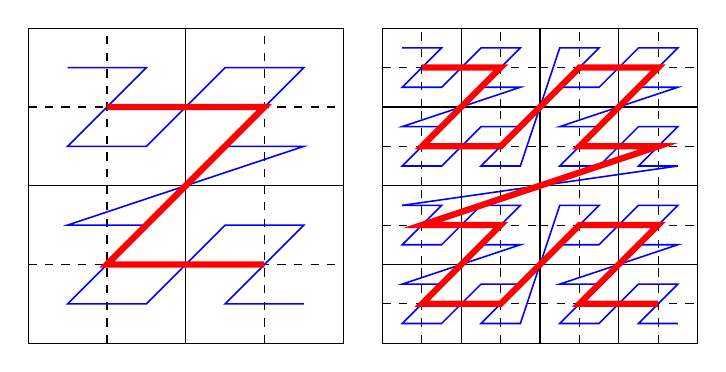
\begin{tikzpicture}
            % First Matrix (0,0) -> (4,4)
            \draw (0,0) rectangle (2,2);
            \draw (2,2) rectangle (4,4);
            \draw (0,2) rectangle (2,4);
            \draw (2,0) rectangle (4,2);
            \draw [dashed] (1,0) -- (1,4);
            \draw [dashed] (3,0) -- (3,4);
            \draw [dashed] (0,1) -- (4,1);
            \draw [dashed] (0,3) -- (4,3);
    
            % Second matrix (4.5,0) -> (8.5,4)
            \foreach \x in {0,...,3} {
                \foreach \y in {0,...,3} {
                    \draw (4.5+\x, \y) rectangle (5.5+\x, 1+\y);
                    \draw [dashed] (4.5+\x, 0.5+\y) -- (5.5+\x, 0.5+\y);
                    \draw [dashed] (5+\x, \y) -- (5+\x, 1+\y);
                }
            }
        
            % Hilbert curve in the first matrix
            \draw [line width=0.2mm, blue] (0.5,3.5) -- (1.5,3.5) -- (0.5,2.5) -- (1.5,2.5) -- (2.5,3.5) -- (3.5,3.5) -- (2.5,2.5) -- (3.5,2.5) -- (0.5,1.5) -- (1.5,1.5) -- (0.5,0.5) -- (1.5,0.5) -- (2.5,1.5) -- (3.5,1.5) -- (2.5,0.5) -- (3.5,0.5);
            \draw [line width=0.8mm, red] (1,3) -- (3,3) -- (1,1) -- (3,1);
            
        
            % Hilbert curve in the second matrix
            \draw [line width=0.2mm, blue, shift={(4.5, 0)}] (0.25, 3.75) -- (0.75, 3.75) -- (0.25, 3.25) -- (0.75, 3.25) -- (1.25, 3.75) -- (1.75, 3.75) -- (1.25, 3.25) -- (1.75, 3.25) -- (0.25, 2.75) -- (0.75, 2.75) -- (0.25, 2.25) -- (0.75, 2.25) -- (1.25, 2.75) -- (1.75, 2.75) -- (1.25, 2.25) -- (1.75, 2.25) -- (2.25, 3.75) -- (2.75, 3.75) -- (2.25, 3.25) -- (2.75, 3.25) -- (3.25, 3.75) -- (3.75, 3.75) -- (3.25, 3.25) -- (3.75, 3.25) -- (2.25, 2.75)-- (2.75, 2.75) -- (2.25, 2.25) -- (2.75, 2.25) -- (3.25, 2.75) -- (3.75, 2.75) -- (3.25, 2.25) -- (3.75, 2.25);
            \draw [line width=0.2mm, blue, shift={(4.5, -2)}] (0.25, 3.75) -- (0.75, 3.75) -- (0.25, 3.25) -- (0.75, 3.25) -- (1.25, 3.75) -- (1.75, 3.75) -- (1.25, 3.25) -- (1.75, 3.25) -- (0.25, 2.75) -- (0.75, 2.75) -- (0.25, 2.25) -- (0.75, 2.25) -- (1.25, 2.75) -- (1.75, 2.75) -- (1.25, 2.25) -- (1.75, 2.25) -- (2.25, 3.75) -- (2.75, 3.75) -- (2.25, 3.25) -- (2.75, 3.25) -- (3.25, 3.75) -- (3.75, 3.75) -- (3.25, 3.25) -- (3.75, 3.25) -- (2.25, 2.75)-- (2.75, 2.75) -- (2.25, 2.25) -- (2.75, 2.25) -- (3.25, 2.75) -- (3.75, 2.75) -- (3.25, 2.25) -- (3.75, 2.25);
            \draw [line width=0.2mm, blue, shift={(4.5, 0)}] (3.75, 2.25) -- (0.25, 1.75);
            \draw [line width=0.8mm, red, shift={(4.5, 0)}] (0.5,3.5) -- (1.5,3.5) -- (0.5,2.5) -- (1.5,2.5) -- (2.5,3.5) -- (3.5,3.5) -- (2.5,2.5) -- (3.5,2.5) -- (0.5,1.5) -- (1.5,1.5) -- (0.5,0.5) -- (1.5,0.5) -- (2.5,1.5) -- (3.5,1.5) -- (2.5,0.5) -- (3.5,0.5);
                    
        \end{tikzpicture}
    }
    \caption{Z-Morton curve projected on a two-by-two, four-by-four and eight-by-eight matrix.}\label{fig:ZMorton}
\end{figure}